\documentclass[a4paper,11pt]{article}
\usepackage{color}
\usepackage{graphicx}
\usepackage{subcaption}
\usepackage{wrapfig}
\usepackage[export]{adjustbox}
\usepackage{geometry}
\usepackage{setspace}
\usepackage{adjustbox}
\usepackage{amsmath}
\usepackage{textgreek}
\usepackage[british]{babel}
\usepackage{url}
\usepackage{siunitx}
\usepackage{textcomp}
\usepackage[square,numbers]{natbib} %the big one
\usepackage{titlepic}
\doublespacing
\geometry{legalpaper, portrait, margin=2cm}
\begin{document}
\title{Open Science Hardware Setup for investigating the Stability of Organic Solar Cells - Interim Report}
\author{Samuel Mendis}
\date{\today}
%%\titlepic{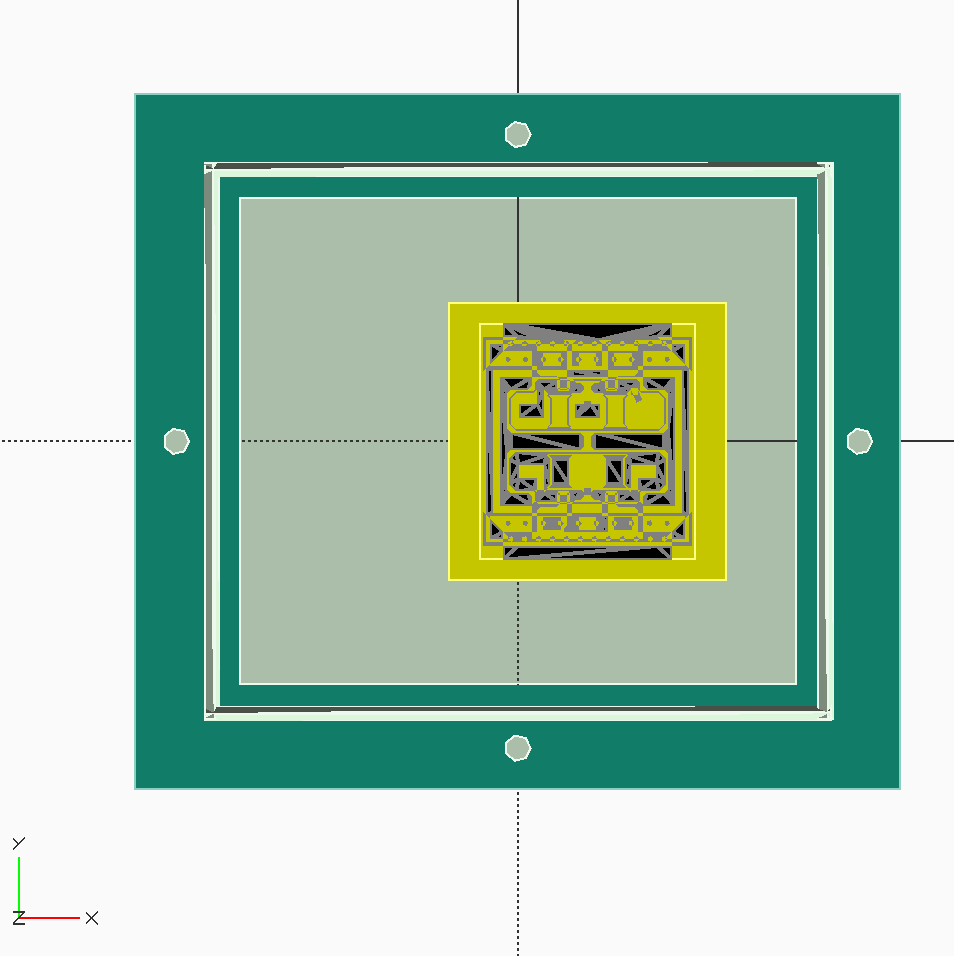
\includegraphics[width=\textwidth]{fig1a}}
\maketitle
\pagebreak
\section{Introduction}
Solar cells are becoming increasingly prevalent in the fight against climate change\cite[p.~XV]{RN45}, leading demand to increase worldwide. This project aims to contribute to the designing of the next generation of solar cells to be manufactured out of organic material (rather than the current industry standard of Silicon). Currently, controlled lifetime testing of organic solar cells is difficult due to the multitude of failure mechanisms. These are caused by chemical degradation via Oxygen and water\cite[p.~689]{RN38}. To combat this problem, this project will design, manufacture and test a programmable lifetime solar testing container. A key tenet of the project is ensuring the accessibility of the research through the use of open hardware in order for the  potential acceleration of the development of organic solar cells.
\section{Aims and Objectives}
The aim of the container is to simulate a lifetime (20 years) of real world degradation in a \emph{reasonable} timeframe. Reasonable means that ideally the testing container should be able to test the solar cell in a short cycle test (15 minutes) or a long multiple cycle test (a period of days). To ensure accurate testing of the cells, the container needs to be airtight. This is to prevent any atmospheric Oxygen and water vapour getting into the container and causing unwanted degradation of the cell. Furthermore, the container should have to have gas inlets and outlets so that the conditions that the solar cell is tested under can be varied. This will be in conjunction with a temperature controller capable of varying the temperature of the solar cell up to 120\textdegree C. These objectives were guided by the paper \emph{Consensus stability testing protocols for organic photovoltaic materials and devices} \cite[p.~1255-1261]{RN47} which cites multiple different testing criteria for an organic solar cell. Additional aims that would enhance the scope of the project is a graphical user interface (GUI) developed to control the conditions within the testing container. These are achievable aims within the timeframe allowed, which can be clearly seen on the Gantt chart attached. 

\section{Progress}\begin{wrapfigure}{b}{0.35\textwidth} 
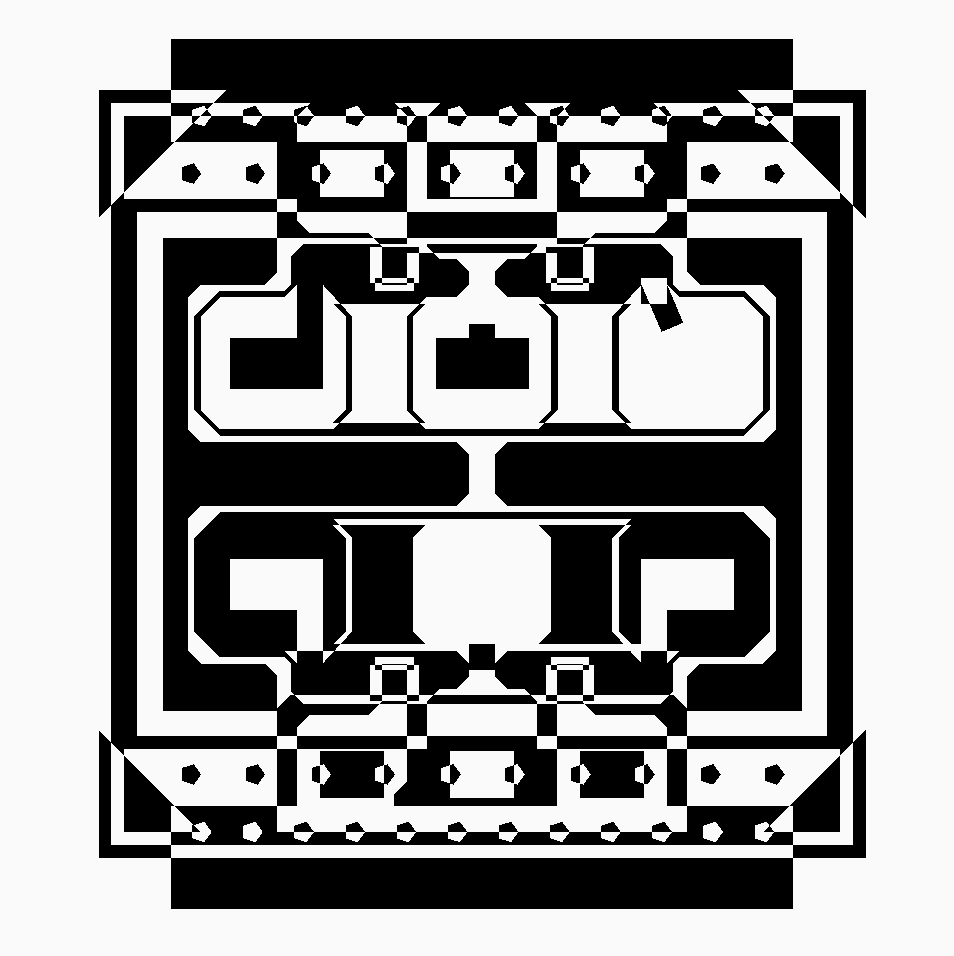
\includegraphics[width=\linewidth]{fig2}
\caption{Model of Substrate provided by Dr. Grey Christophoro\label{fig:substrate}}
\end{wrapfigure}At this stage in the year, the testing container is past the design stage and is onto manufacturing, with the outer shell being cast from AL-xxxx. A full design was completed using the open source software OpenSCAD. Using inspiration from X an AMFD researcher (who had developed a similar type of device, without the functionality) a CAD model of the testing container was built and is shown in Figure \ref{fig:model}.\\ 

\begin{figure}[h]
\begin{subfigure}{0.5\textwidth}
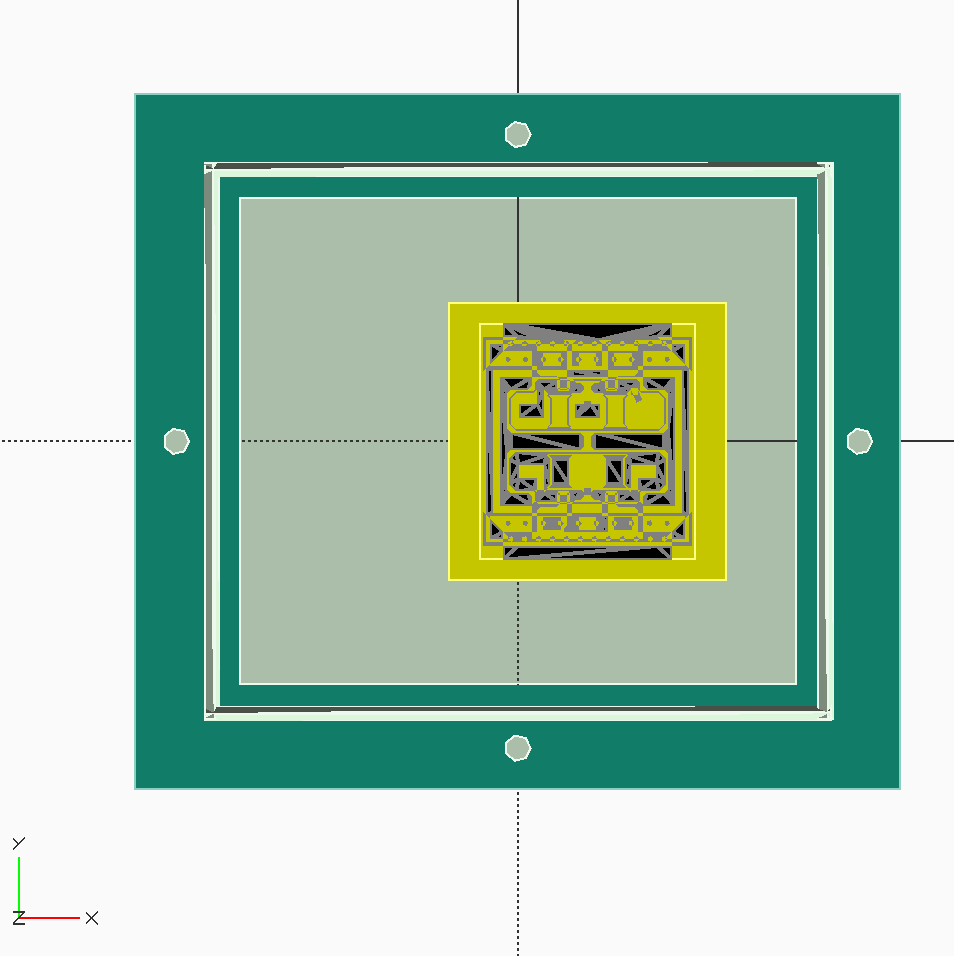
\includegraphics[width=0.9\linewidth]{fig1a}
\caption{Plan View of Model}
\label{fig:subim1}
\end{subfigure} \begin{subfigure}{0.5\textwidth}
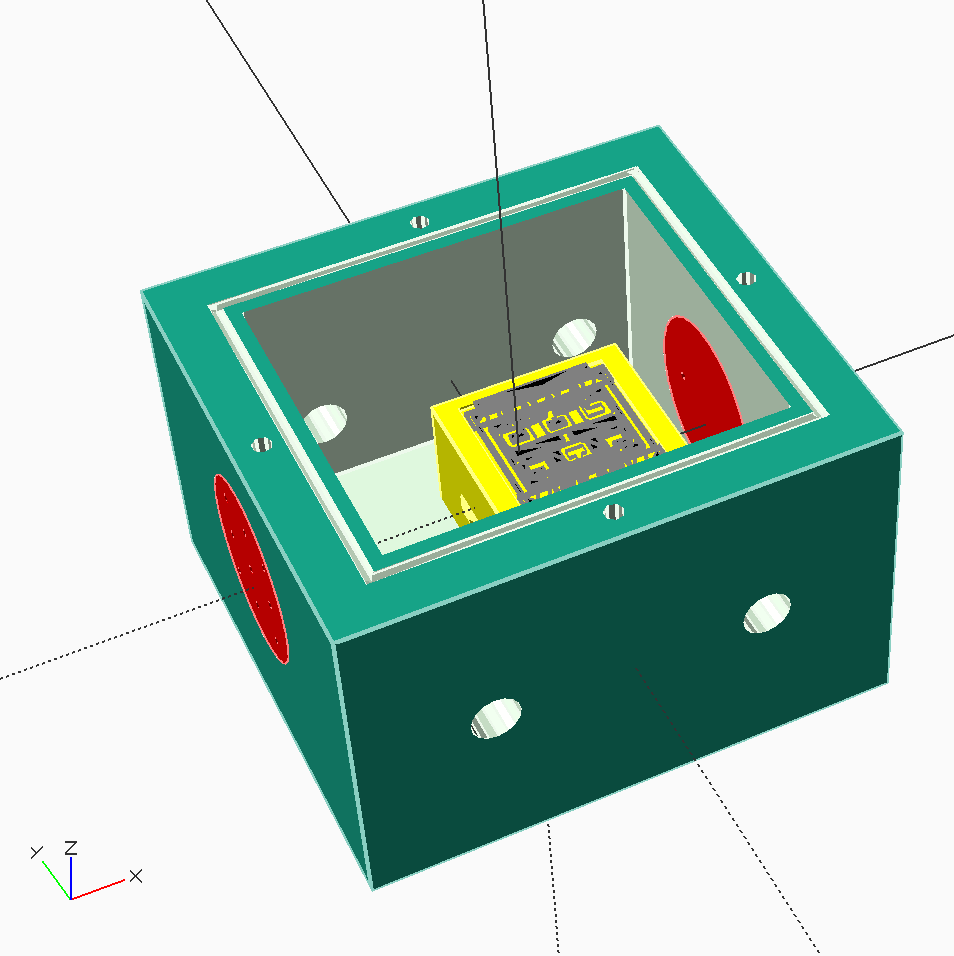
\includegraphics[width=0.9\linewidth]{fig1b}
\caption{Isometric View of Model}
\label{fig:subim2}
\end{subfigure}
\caption{Showing plan and isometric view of the full OpenSCAD model\label{fig:model}}
\label{fig:image2}
\end{figure}
\noindent The three important factors that the container had to accommodate were: the substrate (coloured black in Figure \ref{fig:model}), any electronic devices (temperature controller)  and gas inlet ports. The substrate used carries 8 solar cells with dimensions of 30 mm x 30 mm and a thickness of 1 mm. This can be seen in Figure \ref{fig:substrate} which is a model of the substrate used provided by Dr. Grey Christophoro. In order to carry the substrate in the testing container, a substrate holder (coloured yellow in Figure \ref{fig:model}) was designed to fit within the outer shell of the box allowing a more modular design for the container. This modular design is desirable as it allows the ability to modify which cells and substrate layouts that being tested without the redesign of the entire container, just the substrate holder and associated electronics; thereby saving those who may need to use it in the future valuable time and money. 
\section{Future Work}
Once the outer shell has been manufactured, the next step is to pressure test the vessel. Once confirmed that the vessel is air tight, it will be possible to start working on the control electronics for the systems. This involves calibrating the heating element and temperature sensors as well as creating a controller to modify the environmental conditions. These tasks will require lots of time in the lab to ensure reliability of the container, which is why I have identified it as a potential bottleneck and have planned accordingly. As can be seen from the Gantt chart shown as appendix 1, this section is forecast to take many weeks which as there may be problems when using these components due to a lack of experience. Once the calibration is complete the container will undergo many tests to see if the solar cell reacts as predicted (failing under certain conditions, surviving under inert environments). If this proceeds as predicted in the Gantt chart, the project should be finished by the end of Hillary term, giving 6 weeks contingency if any unforeseen problems crop up. 
\begin{singlespace}
\bibliographystyle{ieeetr} %also the big one 
\bibliography{untitled}

\end{singlespace}
\end{document}